\section{Отчет по лабораторной работы
№1}\label{ux43eux442ux447ux435ux442-ux43fux43e-ux43bux430ux431ux43eux440ux430ux442ux43eux440ux43dux43eux439-ux440ux430ux431ux43eux442ux44b-1}

\subsection{Выбор языков в виртуальной
машине}\label{ux432ux44bux431ux43eux440-ux44fux437ux44bux43aux43eux432-ux432-ux432ux438ux440ux442ux443ux430ux43bux44cux43dux43eux439-ux43cux430ux448ux438ux43dux435}

\begin{figure}
\phantomsection\label{fig:001}
\centering
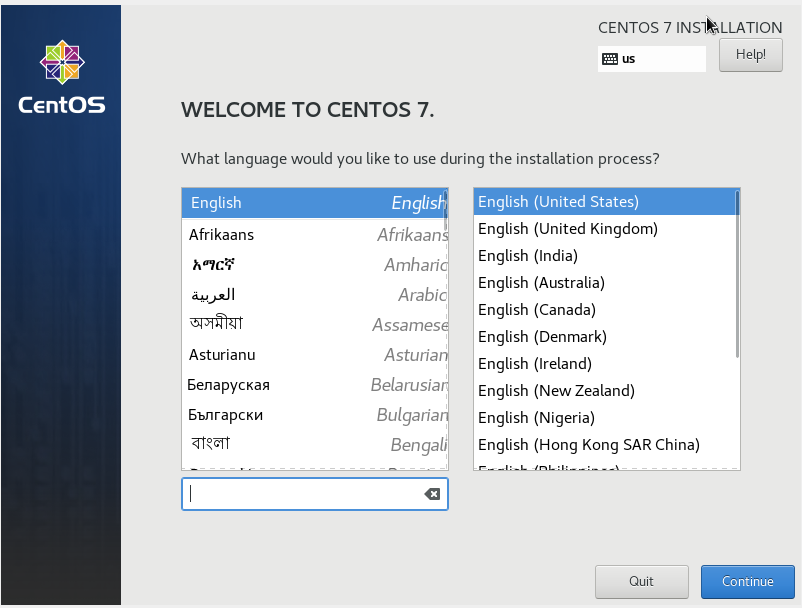
\includegraphics[width=0.7\textwidth,height=\textheight]{image/1.png}
\caption{Выбор языков}\label{fig:001}
\end{figure}

\subsection{Установка виртуальной
машины}\label{ux443ux441ux442ux430ux43dux43eux432ux43aux430-ux432ux438ux440ux442ux443ux430ux43bux44cux43dux43eux439-ux43cux430ux448ux438ux43dux44b}

\begin{figure}
\phantomsection\label{fig:002}
\centering
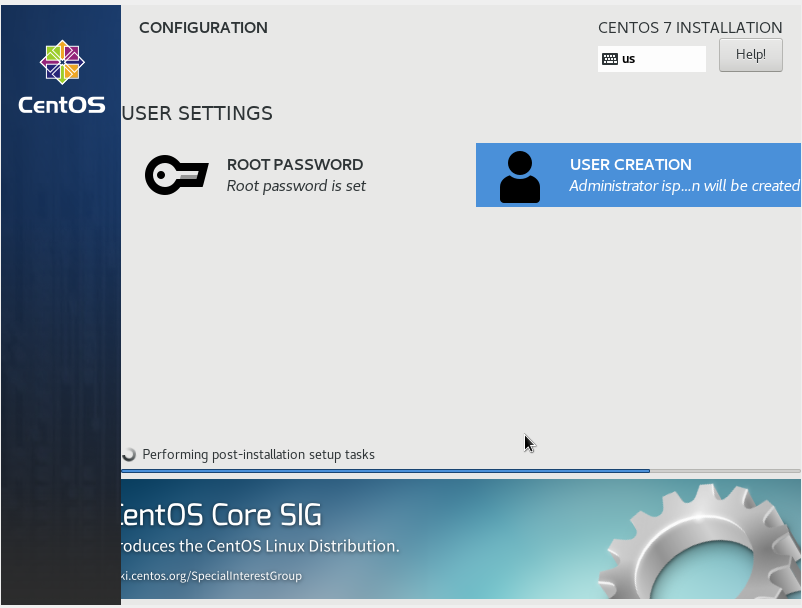
\includegraphics[width=0.7\textwidth,height=\textheight]{image/2.png}
\caption{Установка}\label{fig:002}
\end{figure}

\subsection{Работа с виртуальной машиной (Домашняя работа
№1)}\label{ux440ux430ux431ux43eux442ux430-ux441-ux432ux438ux440ux442ux443ux430ux43bux44cux43dux43eux439-ux43cux430ux448ux438ux43dux43eux439-ux434ux43eux43cux430ux448ux43dux44fux44f-ux440ux430ux431ux43eux442ux430-1}

\begin{itemize}
\tightlist
\item
  На данном слайде представлено одно из заданий Домашней работы к
  лабораторной работе №1
\end{itemize}

\begin{figure}
\phantomsection\label{fig:003}
\centering
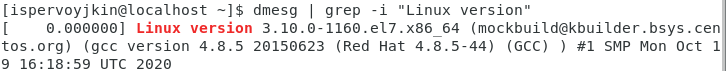
\includegraphics[width=0.7\textwidth,height=\textheight]{image/3.png}
\caption{Задание}\label{fig:003}
\end{figure}

\subsection{Основные команды
git}\label{ux43eux441ux43dux43eux432ux43dux44bux435-ux43aux43eux43cux430ux43dux434ux44b-git}

\begin{itemize}
\tightlist
\item
  На данном скриншоте представлены команды git, которые позволяют
  конфигурировать git на компьютере
\end{itemize}

\begin{figure}
\phantomsection\label{fig:004}
\centering
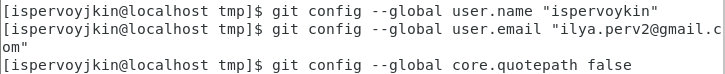
\includegraphics[width=0.7\textwidth,height=\textheight]{image/4.png}
\caption{Задание}\label{fig:004}
\end{figure}

\subsection{Работа с
Markdown}\label{ux440ux430ux431ux43eux442ux430-ux441-markdown}

\begin{itemize}
\tightlist
\item
  На данных скриншотах представлены команды, которые позволяют
  преобразовать файл .markdown в файлы .pdf и .docx соответственно
\end{itemize}

\begin{figure}
\phantomsection\label{fig:005}
\centering
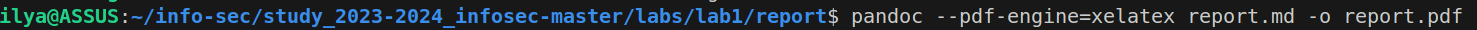
\includegraphics[width=0.7\textwidth,height=\textheight]{image/5.png}
\caption{Задание}\label{fig:005}
\end{figure}

\begin{figure}
\phantomsection\label{fig:006}
\centering
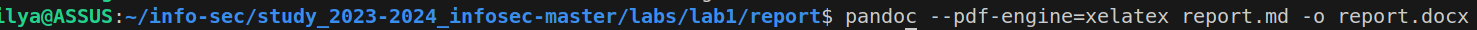
\includegraphics[width=0.7\textwidth,height=\textheight]{image/6.png}
\caption{Задание}\label{fig:006}
\end{figure}

\subsection{Выводы}\label{ux432ux44bux432ux43eux434ux44b}

\begin{itemize}
\tightlist
\item
  Установил VirtualBox, изучил её работу.
\item
  Изучил идеологию и научился применять средства контроля версий.
\item
  Научился работать с Markdown-файлами.
\item
  Научился создавать pdf и docx файлы из файла Markdown (с помощью
  команды make);
\end{itemize}
